\chapter{Considerações finais}
Este projeto foi desenvolvido ao longo do ano de 2017, a Figura \ref{horas-trabalhadas} mostra a quantidade de horas trabalhada.

\begin{figure}[H]
\caption{\label{horas-trabalhadas} Controle horas trabalhadas}
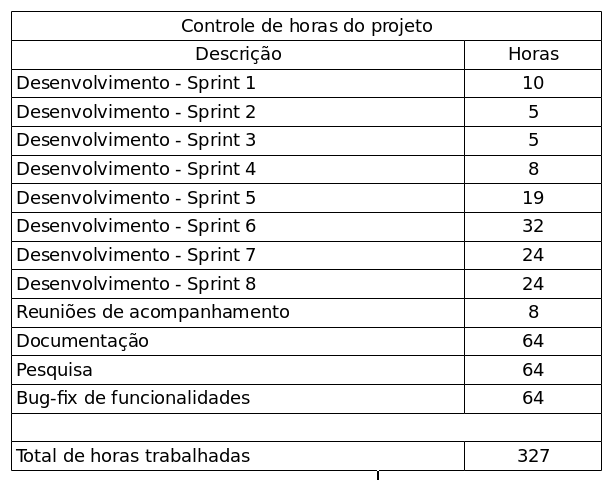
\includegraphics[scale=0.4]{img/horas-trabalhadas.png}
\legend{Fonte: Autor do projeto}
\end{figure}

Foi uma atividade que envolveu pesquisa, gerenciamento de tempo e criatividade, nem sempre tudo ocorre como planejado e fazer adaptações e descobrir melhores soluções fizeram parte desta atividade. Ao longo do desenvolvimento deste projeto muitas idéias e conceitos interessantes foram descobertos, mas nem sempre foi possível adiciona-los ao projeto, por isso é importante ao menos cita-los como uma referencia para implementações futuras.

\section{Funcionalidades futuras}
Estas funcionalidades foram separadas em dois grupos.

\subsection{Segurança}
Toda informação deveria estar transitando em um meio seguro para troca de mensagens, no caso a utilização do protocolo http com sua camada de segurança em ssl, isso envolve o serviço da API e a troca de mensagens do \textit{broker} no protocolo mqtt.

\subsection{Hospedagem em servidor externo}
Hospedar em um serviço externo traria a possibilidade de controlar os dispositivos de casa em qualquer lugar onde os usuários pudessem acessar a internet. A dificuldade estava em fazer um aplicativo que soubesse "chavear" entre uma rede local e um serviço na web, com o uso de \textit{Progressive Web Apps} (PWA) a mesma estrutura de aplicativo web instalado na central de controle funcionaria para controle usando o serviço hospedado. Outro ponto que seria necessário lidar, o \textit{broker} precisa existir no serviço remoto, isso poderia ser resolvido com a criação de \textit{containers} Docker com a mesma infraestrutura da central de controle. Nos teste realizados durante o TCC-1 foi feito a ligação do \textit{broker} local com um \textit{broker} remoto, estas tentativas foram deixadas de lado visando um produto mínimo viável.

\subsection{Mais opções de dispositivos}
Atualmente a API sabe lidar apenas com o acionamento de relés, seria muito interessante adicionar funcionalidades como acionamento por \textit{timer}, leitura de sensores de temperatura e detecção de presença.



